\documentclass[a4paper,11pt]{article}

\usepackage{pdflscape}

%% Latex documents that need direct input
%% Stuff for MARIE CURIE
\usepackage[T1]{fontenc}
\usepackage{lmodern}
\usepackage{eurosym}
\usepackage{lastpage}
\usepackage{xspace}
\usepackage[margin=16mm,includehead,includefoot]{geometry}
\usepackage{fancyhdr}
\usepackage{booktabs}
\usepackage{multirow}
\usepackage{array}
\usepackage[table]{xcolor}
\usepackage{csquotes}
\usepackage{pgfgantt}
\usepackage{titlesec} % fancy titles for sections, subsections etc..
\usepackage[style=verbose-ibid,backend=bibtex]{biblatex}
\usepackage{amssymb}
%% Regular stuff

%  The following command loads a graphics package to include images
%  in the document. It may be necessary to specify a DVI driver option,
%  e.g., [dvips], but that may be inappropriate for some LaTeX
%  installations.
\usepackage[]{graphicx}

% In order to include files without having a clear page using \include*,
% the newclude package is required
\usepackage{newclude}

% Required for acronyms
% use \acresetall to reset the acroyms counter
% macros=True, allows for calling \myTriger rather than \ac{myTriger}
% \usepackage[single=true, macros=true, xspace=true]{acro}

% Use biblatex to manage the referencing
%
% \usepackage[style=verbose-ibid,backend=bibtex]{biblatex}
% \usepackage[style=authoryear,backend=biber]{biblatex}

% Clever cross referencing. Using cleverref, instead of writting
% figure~\ref{...} or equation~\ref{...}, only \cref{...} is required.
% The package interprates the references and introduces the figure, fig.,
% equation, eq., etc keywords. \Cref forces first letter capital.
% >> WARNING: This package needs to be loaded after hyperref, math packages,
%             etc. if used.
%             Cleveref is recomended to load late
\usepackage{hyperref}
\usepackage{cleveref}

% To create random text use lipsum
\usepackage{lipsum}
        % contains the latex packages
% \title{Some \LaTeX{} template in various forms}
% \author{Andrew Author and Ben Author}


\newcommand{\proposalAcronym}{{PREDICATE}\xspace}

%% Choose the appropiated evaluation pannel
\newcommand{\evaluationPannel}{{Standard GF}\xspace}
% \newcommand{\evaluationPannel}{{Standard EF}\xspace}
% \newcommand{\evaluationPannel}{{\sc CAR}\xspace}
% \newcommand{\evaluationPannel}{{\sc RI}\xspace}
             % contains the information regarding Project call, title, autor, etc.
%%%%%%%%%%%%%%%%%%%%%%%%%%%%%%%%%%%%%%%%%%%%%%%%%%%%%%%%%%%%% 
%>>>> uncomment following for page numbers
% \pagestyle{plain}    
%>>>> uncomment following to start page numbering at 301 
%\setcounter{page}{301} 

\renewcommand{\familydefault}{\sfdefault}
\normalfont % this is required for the change to take effect

\newcommand{\TODO}[1]{{\textcolor{red}{[\textbf{TODO:} #1]}}}
\titlespacing\section{0pt}{6pt plus 4pt minus 2pt}{0pt plus 2pt minus 2pt}
\titlespacing\subsection{0pt}{6pt plus 4pt minus 2pt}{0pt plus 2pt minus 2pt}
\titlespacing\subsubsection{0pt}{6pt plus 4pt minus 2pt}{0pt plus 2pt minus 2pt}

\titleformat*{\section}{\large\bfseries}
\titleformat*{\subsection}{\normalsize\bfseries}
\titleformat*{\subsubsection}{\normalsize\bfseries}
\let\oldfootnotesize\footnotesize
% \renewcommand{\footnotesize}{\fontsize{8bp}{1em}\selectfont}
% \renewcommand{\cite}{\autocite} % citations in footnotes
% \bibliography{bibliography}

\headheight=14pt

\hypersetup{
    pdftitle={H2020-MSCA-IF-2015},    % title
    pdfauthor={xxxxxxxxx},
    colorlinks=true,
    citecolor=black,
    linkcolor=black,
    urlcolor=blue
  }

\pagestyle{fancy}
\fancyhead{}
\fancyhead[C]{{\sc \proposalAcronym}\,--\,\evaluationPannel}
\fancyfoot{}
\fancyfoot[C]{Part B - Page \thepage~of \pageref{LastPage}}


\renewcommand{\headrulewidth}{0pt}


\renewcommand{\contentsname}{TABLE OF CONTENTS}

      % contains package and variables init.
%% Acronym definition example using glossaries package
%% \usepackage{acro} is required
%% 
%% For a powerful usage of the acro package look at http://tex.stackexchange.com/questions/135975/how-to-define-an-acronym-by-using-other-acronym-and-print-the-abbreviations-toge

\DeclareAcronym{us}{
  short = US,
  long  = Ultra-Sound
}

\DeclareAcronym{cad}{
  short = CAD,
  long  = Computer-Aided Diagnosis
}

\DeclareAcronym{dm}{
  short = DM,
  long  = Digital Mammography
}

\DeclareAcronym{gt}{
  short = GT,
  long  = Ground Truth
}

\DeclareAcronym{bus}{
%  short = B\acs*{us},
%  long  = Breast \acifused{us}{\acs*{us}}{\acl*{us}}
short = BUS,
long= Breast Ultra-Sound
}

\DeclareAcronym{ml}{
  short = ML,
  long  = Machine Learning
}

\DeclareAcronym{svm}{
  short = SVM,
  long  = Support Vector Machines
}

\DeclareAcronym{acm}{
  short = ACM,
  long  = Active Contour Model
}

\DeclareAcronym{crf}{
  short = CRFs,
  long  = Conditional Random Fields
}

\DeclareAcronym{mrf}{
  short = MRFs,
  long  = Markov Random Fields
}

\DeclareAcronym{cv}{
  short = CV,
  long  = Computer Vision
}
\DeclareAcronym{icm}{
  short = ICM,
  long  = Iterated Conditional Modes
}
\DeclareAcronym{sa}{
  short = SA,
  long  = Simulate Anealing
}
\DeclareAcronym{gc}{
  short = GC,
  long  = Graph-Cuts
}

\DeclareAcronym{aov}{
  short = AOV,
  long  = Area Overlap
}

\DeclareAcronym{birads}{
  short = BI-RADS,
  long  = Breast Imaging-Reporting and Data System
}

\DeclareAcronym{mad}{
  short = MAD,
  long  = Median Absolute Deviation
}

\DeclareAcronym{qc}{
  short = QC,
  long  = Quadratic-Chi
}

\DeclareAcronym{sift}{
  short = SIFT,
  long  = Self-Invariant Feature Transform
}

\DeclareAcronym{bof}{
  short = BoF,
  long  = Back-of-Features
}

\DeclareAcronym{fa}{
  short = FA,
  long  = Fibro-Adenoma
}

\DeclareAcronym{dic}{
  short = DIC,
  long  = Ductal Inflating Carcinoma
}

\DeclareAcronym{ilc}{
  short = ILC,
  long  = Inflating Lobular Carcinoma
}

\DeclareAcronym{fpr}{
  short = FPR,
  long  = False Positive Ratio
}

\DeclareAcronym{fnr}{
  short = FNR,
  long  = False Negative Ratio
}

\DeclareAcronym{fp}{
  short = FP,
  long  = False Positive
}

\DeclareAcronym{rbf}{
  short = RBF,
  long  = Radial Basis Function
}

\DeclareAcronym{mri}{
  short = MRI,
  long  = Magnetic Resonance Imaging
}

\DeclareAcronym{erspc}{
  short = ERSPC,
  long  = European Randomised Study of Screening for Prostate Cancer
}

\DeclareAcronym{psa}{
  short = PSA,
  long  = Prostate-Specific Antigen
}

\DeclareAcronym{t2w}{
  short = T\textsubscript{2}-W,
  long  = T\textsubscript{2}-Weighted
}

\DeclareAcronym{dce}{
  short = DCE,
  long  = Dynamic Contrast-Enhanced
}

\DeclareAcronym{dw}{
  short = DW,
  long  = Diffusion Weighted
}

\DeclareAcronym{adc}{
  short = ADC,
  long  = Apparent Diffusion Coefficient
}

\DeclareAcronym{mrsi}{
  short = MRSI,
  long  = Magnetic Resonance Spectroscopy Imaging
}

\DeclareAcronym{pz}{
  short = PZ,
  long  = Peripheral Zone
}

\DeclareAcronym{cg}{
  short = CG,
  long  = Central Gland
}

\DeclareAcronym{cnn}{
  short = CNN,
  long  = Convolutional Neural Networks
}

\DeclareAcronym{asm}{
  short = ASM,
  long  = Active Shape Models
}

\DeclareAcronym{pirads}{
  short = PI-RADS,
  long  = Prostate Imaging and Reporting and Data System
}

\DeclareAcronym{acr}{
  short = ACR,
  long  = American College of Radiology
}

\DeclareAcronym{esur}{
  short = ESUR,
  long  = European Society of Urogenital Radiology
}

\DeclareAcronym{fsu}{
  short = FSU,
  long  = Florida State University
}

\DeclareAcronym{udg}{
  short = UdG,
  long  = Universitat de Girona
}

\DeclareAcronym{roc}{
  short = ROC,
  long  = Receiver Operating Characteristic
}
      % contains the acronyms

%% Select inputing only one part of the document
%\includeonly{./content/participants/list}   % the file wihtout .tex
%\includeonly{./content/proposal/excelence}
%\includeonly{./content/proposal/impact}
%\includeonly{./content/proposal/implementation}
%\includeonly{./content/cv/cv}

\addbibresource{./content/lit_review.bib}

\begin{document}
\phantom{a}
\vspace{15mm}
\begin{center}


        \Large{


        \textbf{START PAGE}

          \vspace{15mm}
          MARIE SK\L{}ODOWSKA-CURIE ACTIONS\\
          \vspace{1cm}

          \textbf{Individual Fellowships (IF)}\\
          \textbf{Call: H2020-MSCA-IF-2015}
          \vspace{2cm}

          PART B
          \vspace{2.5cm}

          ``\proposalAcronym''\\
          \vspace{1cm}
          ``Deep-learning based multi-parametric MRI computer-aided diagnosis for prostate cancer''
          \vspace{1cm}

          \textbf{This proposal is to be evaluated as:}
          \vspace{.5cm}

          \textbf{\evaluationPannel}
        }

  \end{center}
\vspace{1cm}



\newpage
\setcounter{tocdepth}{1}
\setcounter{section}{-1}
\tableofcontents


\section{LIST OF PARTICIPANTS}
\label{sec:participants}

\newcommand\rotx[1]{\rotatebox[origin=c]{90}{\textbf{#1}}}
\newcommand\roty[1]{\rotatebox[origin=c]{90}{\parbox{4cm}{\raggedright\textbf{#1}}}}
\newcommand\MyHead[2]{\multicolumn{1}{l|}{\parbox{#1}{\centering #2}}}

\renewcommand{\arraystretch}{2}
\noindent\begin{tabular}{|m{2.4cm}|m{1cm}|b{1em}|b{1em}|c|m{2.5cm}|m{2cm}|c|}
\rowcolor{lightgray}
\hline
  \textbf{Participants}
& \MyHead{1cm}{\cellcolor{lightgray}\textbf{Legal\\Entity\\Short\\Name}}
& \rotx{Academic}
& \rotx{Non-academic}
& \textbf{Country}
& \MyHead{2.1cm}{\cellcolor{lightgray}\textbf{Dept. / \\Division / \\Laboratory}}
& \textbf{Supervisor}
& \MyHead{2.5cm}{\textbf{Role of\\Partner\\Organisation}} \\
\hline
\underline{Beneficiary} & & & & & & & \\\hline
Universitat de Girona  & UdG & \checkmark & & Spain & Computer Vision and Robotics Institute (ViCOROB) & Dr. Robert Mart\'i & \\\hline   % Add \checkmark where applicable.
\underline{Partner} \underline{Organisation} & & & & & & & \\\hline
Florida State University  & FSU & \checkmark & & USA & Scientific Computing & Prof. A. Meyer-Baese & Host outgoing phase \\\hline
\end{tabular}
\renewcommand{\arraystretch}{1}
\vspace{\baselineskip}

% Data for non-academic beneficiaries

% \noindent\begin{tabular}{|m{1.7cm}|m{2cm}|m{1.8cm}|c|c|m{2.5cm}|c|c|c|}
% \hline
%   \textbf{Name}
% & \roty{Location of research premises (city / country)}
% & \roty{Type of R\&D activities}
% & \roty{No. of fulltime employees}
% & \roty{No. of employees in R\&D}
% & \roty{Website}
% & \roty{Annual turnover (approx. in Euro)}
% & \roty{Enterprise status (Yes/No)}
% & \roty{SME status  (Yes/No)}
% \\\hline
% & & & & & & & & \\\hline
% \end{tabular}
% \vspace{\baselineskip}

Note that:
\begin{itemize}
\item Any inter-relationship between different participating institutions or individuals (e.g. family ties, shared premises or facilities, joint ownership, financial interest, overlapping staff or directors, etc.) must be declared and justified in this part of the proposal;
\item The information in the table for non-academic beneficiaries must be based on current data, not projections;
\item The data provided relating to the capacity of the participating institutions will be subject to verification during the Grant Agreement preparation phase.
\end{itemize}
                 % the file wihtout .tex

\newpage
%\section{SUMMARY}
%\label{sec:summary}
% Hiiiii \us is \ac{us} then \us is xx
% Please provide a short summary of the proposal, which could be the same as the proposal abstract, built around a research/innovation project.

% Regular citation~\cite{Xarticle} and a footnote citation~\footcite{Xbook}.

% Here all the citations need to be footnote but own publications, etc. should belong to the text.
% Look at the source-code for the hack.

% \let\citeBk=\cite
% \let\cite=\footcite

% Now both should bee a footnote. This is regular citation~\cite{Xarticle_full} and a footnote citation~\footcite{Xbook_full}.

% \let\cite=\citeBk

% Back to regular behaviour. This is regular citation~\cite{Xarticle_full} and a footnote citation~\footcite{Xbook_full}.

\let\citeBk=\cite
\let\cite=\footcite
\renewcommand{\footnotesize}{\scriptsize}

That will be the abstract of the proposal

%% Incldue the content without .tex extension
% \acresetall  % reset the acronyms from the abstract
\include*{./content/proposal/excellence}               % the file wihtout .tex
\include*{./content/proposal/impact}                  % the file wihtout .tex
\include*{./content/proposal/implementation}          % the file wihtout .tex
\section{CV OF THE EXPERIENCED RESEARCHER}
\label{sec:cv}

\setlength{\parindent}{0cm}{

\subsection{PERSONAL INFORMATION}

\emph{Name}: Guillaume Lema\^itre \\
\emph{Date of birth}: 27\textsuperscript{th} April 1988, 27 years old \\
\emph{Personal website}: \texttt{https://sites.google.com/site/glemaitre58} \\

\subsection{EDUCATION}

\begin{table}[!h]
\begin{tabular}{p{4cm} p{13cm}}
 \\
\textbf{07/2012 --- 12/2015} & \textbf{Co-joint PhD in Medical Imaging} \\
& \textit{``Computer Aided Diagnosis system for prostatic biopsy guidance and follow-up fusing multi-modal imaging''} \\
& Supervised by Dr. R. Mart\'i, Prof. F. M\'eriaudeau, Dr. J. Freixenet, and Dr. P. M. Walker \\
& ViCOROB, Universitat de Girona --- LE2I, Universit\'e de Bourgogne \\[.5em]  \\
\textbf{09/2012 --- 09/2014} & \textbf{Master in Business Innovation and Technology Management} \\
& \textit{``Valorisation of computerized technology in the health care sector''} \\
& Supervised by Dr. A. Bikfalvi and Dr. J. Llach \\
& Universitat de Girona \\[.5em]  \\
\textbf{09/2009 --- 06/2011} & \textbf{Master of Excellence Erasmus Mundus in Vision and Robotics} \\
& \textit{``Absolute Quantification in 1H MRSI of the Prostate at 3.0 T''} \\
& Supervised by Dr. P. M. Walker \\
& Universit\'e de Bourgogne, Universitat de Girona, Heriot-Watt University \\[.5em]  \\
\textbf{09/2016 --- 09/2009} & \textbf{Bachelor Eng. Electronic, Signal, and Image} \\
& Universit\'e de Bourgogne \\[.5em]  \\
\end{tabular}
\end{table}

\subsection{WORKING EXPERIENCE}

\begin{table}[!h]
\begin{tabular}{p{4cm} p{13cm}}
 \\
\textbf{03/2015 --- 01/2016} & \textbf{Assistant professor (ATER)} \\
& 184 hours of lecturing in databases, pattern recognition and machine learning, programming, image processing \\
& Universit\'e de Bourgogne \\[.5em]  \\
\textbf{06/2011 --- 06/2012} & \textbf{R\&D researcher} \\
& Barcelona Digital --- ViCOROB, Universitat de Girona \\[.5em]  \\
\end{tabular}
\end{table}

\subsection{FELLOWSHIPS AND AWARDS}

\begin{table}[!h]
\begin{tabular}{c p{14cm}}
2012 & \textbf{OMJ Grant}, Minit\`ere Fran\c cais des Affaires Etrang\`eres et Europ\'eennes, France\\
2012 & \textbf{FI-DGR PhD Grant}, Generalitat de Catalunya - AGAUR, Spain\\
2011 & \textbf{Research Master Scholarship}, Burgundy Region, France\\
2010 & \textbf{Erasmus Spanish Scholarship}, Spanish Ministry, Spain\\
2010 & \textbf{Merit-based Scholarship}, French Ministry, France\\
2010 & \textbf{Merit-based Scholarship dedicated to Research Masters}, Burgundy Region, France\\
2009 & \textbf{Spanish Ministry Mobility Scholarship}, Spanish Ministry, Spain\\
2009 & \textbf{Merit-based Scholarship}, French Ministry, France\\
2009 & \textbf{Erasmus French Scholarship}, French Ministry, France\\
2009 & \textbf{Mobility Grant}, Burgundy Region, France\\
2009 & \textbf{Region Mobility Scholarship}, Burgundy Region, France\\
2009 & \textbf{Rotary Scholarship}, Rotary Club Le Creusot, France\\
2009 --- 2011 & \textbf{Erasmus Mundus Grant}, Heriot-Watt University, Universitat de Girona, Universit\'e de Bourgogne, Scotland, Spain, France\\
2008 & \textbf{Erasmus French Scholarship}, French Ministry, France\\
2008 & \textbf{Mobility Grant}, Burgundy Region, France
\end{tabular}
\end{table}

\begin{table}[!h]
\begin{tabular}{c p{14cm}}
July, 2008 & \textbf{Student Autonomous Underwater Competition - Europe}, Nessie III - Heriot-Watt University \\
July, 2008 & \textbf{THALES Special Award for innovation}, Nessie III - Heriot-Watt University
\end{tabular}
\end{table}

\subsection{PARTICIPATION IN PUBLIC-FUNDED PROJECTS}

\begin{itemize}
\item Temporal analysis and automatic detection of lesions in multi-modal images (IA-BioBreast)
\item OCT imaging
\item Erasmus+ Early Mastery project
\end{itemize}

\subsection{TEACHING}

\begin{table}[!h]
\begin{tabular}{c p{13cm}}
\textbf{24 h} & \textbf{Medical Imaging: Segmentation and registration methods} \\
& Master Erasmus Mundus ViBOT \\
& Universitat de Girona \\
\textbf{24 h} & \textbf{Pattern Recognition and Machine Learning} \\
& Master Erasmus Mundus ViBOT \\
& Universit\'e de Bourgogne  \\
\textbf{48 h} & \textbf{Introduction to image processing} \\
& Master Erasmus Mundus ViBOT \\
& Universit\'e de Bourgogne  \\
\textbf{16 h} & \textbf{Software engineering} \\
& Master Erasmus Mundus ViBOT \\
& Universit\'e de Bourgogne   \\
\textbf{74 h} & \textbf{Introduction to databases} \\
& Bachelor of Electrical Engineering \\
& Universit\'e de Bourgogne  \\
\end{tabular}
\end{table}

\subsection{SUPERVISION}

\begin{itemize}
\item Supervision of 3 BSc. and MSc. students during their summer internships
\end{itemize}

\subsection{PUBLICATIONS}

\underline{\textit{Peer-Review Journals Papers:}}

\begin{enumerate}
\item \textbf{G. Lemaitre, R. Marti, J. Freixenet, J. C. Vilanova, P. M. Walker, and F. Meriaudeau}, ``Computer-Aided Detection and Diagnosis for prostate cancer based on mono and multi-parametric MRI: A Review'', \textit{Computer in Biology and Medicine}, vol. 60, pp 8 - 31, 2015. \textbf{(Citations: 3)}
\end{enumerate}

\underline{\textit{Peer-Review International Conferences Papers:}}

\begin{enumerate}
\item \textbf{A. Meyer-Baese, J. Massich, G. Lemaitre, and M. Rastgoo}, ``Real-Time Optical Flow with Theoretically Justified Warping Applied to Medical Imaging'', \textit{Breast Image Analysis Workshop (BIA), Medical Image Computing and Computer Assisted Interventions (MICCAI) 2015}. Munich: Germany (Oct. 2015). \textbf{(Citations: 0)}
\item \textbf{J. Massich, G. Lemaitre, J. Marti and F. Meriaudeau}, ``An Optimization Approach to Segment Breast Lesions in Ultra-Sound Images using Clinically Validated Visual Cues'', \textit{Breast Image Analysis Workshop (BIA), Medical Image Computing and Computer Assisted Interventions (MICCAI) 2015}. Munich: Germany (Oct. 2015). \textbf{(Citations: 0)}
\item \textbf{G. Lemaitre, M. Rastgoo, J. Massich, S. Sankar, F. Meriaudeau, and D. Sidibe}, ``Classification of SD-OCT volumes with LBP: Application to DME detection'', \textit{Ophthalmic Medical Image Analysis Workshop (OMIA), Medical Image Computing and Computer Assisted Interventions (MICCAI) 2015}. Munich: Germany (Oct. 2015). \textbf{(Citations: 0)}
\item \textbf{J. Massich, G. Lemaitre, J. Marti, and F. Meriaudeau}, ``Brest Ultra-Sound image Segmentation: an Optimization approach based on super-pixels and high-level descriptors'', \textit{International Conference on Quality Control and Artificial Vision (QCAV) 2015}. Le Creusot: France (Jun. 2015). \textbf{(Citations: 0)}
\item \textbf{G. Lemaitre, J. Massich, R. Marti, J. Freixenet, J. C. Vilanova, P. M. Walker, D. Sidibe, and F. Meriaudeau}, ``A Boosting Approach for Prostate Cancer Detection using Multi-parametric MRI'', \textit{International Conference on Quality Control and Artificial Vision (QCAV) 2015}. Le Creusot: France (Jun. 2015). \textbf{(Citations: 0)}
\item \textbf{G. Lemaitre, A. Bikfalvi, J. Llach, J. Massich, and F. Julian}, ``Business Model Design for University Technology Valorisation'', \textit{International Technology, Education and Development Conference (INTED) 2015}. Madrid: Spain (Mar. 2015). \textbf{(Citations: 0)}
\item \textbf{M. Rastgoo, G. Lemaitre, X. Rafael, F. Miralles, and P. Casale}, ``Pruning AdaBoost for Continuous Sensors Mining Applications'', \textit{Ubiquitous Data Mining Workshop, 20th European Conference in Artificial Intelligence 2012}. Montpellier: France (Aug. 2012). \textbf{(Citations: 2)}
\item \textbf{G. Lemaitre, E. Vargiu, J.A. Lorenzo Fernández, and F. Miralles}, ``Real-Time 2D Face Detection and Features-based Tracking in Video'', \textit{IADIS Multi Conference in Computer Science in Computer Graphics, Visualization, Computer Vision and Image Processing 2012}. Lisbon: Portugal (Jul. 2012), 2012. \textbf{(Citations: 0)}
\item \textbf{J. Cartwright, N. Johnson, B. Davis, Z. Qiang, T.L. Bravo, A. Enoch, G. Lemaitre, H. Roth, and Y. Petillot}, ``Nessie III Autonomous Underwater Vehicle for SAUC-E 2008'', \textit{The Unmanned Underwater Vehicle Showcase (UUVS)}, 2008. \textbf{(Citations: 5)}
\end{enumerate}

}                             % the file wihtout .tex
\section{CAPACITIES OF THE PARTICIPATING ORGANISATIONS}
\label{sec:capacities}

\vspace{\baselineskip}

{\fontsize{9bp}{1em}\selectfont % should be 9pt
\noindent\begin{tabular}{>{\raggedright}p{.25\textwidth}p{.7\textwidth}}
  \multicolumn{2}{l}{\textbf{Beneficiary ViCOROB research institute (Universitat de Girona)}} \\\midrule
\textbf{General Description} &
ViCOROB research institute belongs to the Department d'Aquitectura i Technologia de Computadors at the Universitat de Girona, a public university in Girona since 1992. ViCOROB is a research institute specialized in computer vision and robotics at \ac{udg}. In 2013, the \ac{udg} has rewarded ViCOROB by promoting the group into a Research Institute funded by the university itself.
VICOROB has been always highly motivated to solve different and challenging  societal problems and succeeded to obtain outside funding for solving them. The scientific results have been disseminated not only in form of peer-reviewed articles but also to the broad public audience by participating in several media events, speeches and published material. Three spin-off companies emerged: Coronis Computing SL, AQSENSE and BonesNotes.
\\\midrule
\textbf{Role and Commitment of key persons (supervisor)} &
Dr. Robert Mart\'i, PhD, is associate professor in the Image Analysis Lab within ViCOROB. His main research interests are in the field of medical image analysis, specially focusing on feature extraction, pattern-recognition and image registration and its application to mammographic and prostate image analysis and \ac{cad} system.
\\\midrule
\textbf{Key Research Facilities, Infrastructure and Equipment} &
The laboratories of ViCOROB are well-equipped with computers, servers, and specific software required for processing clinically data acquired. The Image Analysis Lab has recently been equipped with 2 high-performance servers (featuring 4 quad-core processors and 128 GB of RAM), a Totoku MS31i2 Diagnostic Displays system, and access to the use of CESCA facilities (the Supercomputing research center in Barcelona) which offers supercomputing shared-memory and distributed-memory machines suitable when dealing with such huge amount of data.
\\\midrule
\textbf{Independent research premises?} &
Yes --- 2 clusters with 32 nuclei for massive and parallel computing
\\\midrule
\textbf{Previous Involvement in Research and Training Programmes} &
During the last 3 years, \ac{udg} has coordinated 6 individual MCA and 2 Research Networks (RESKITCHLAB and CHEMEVE). In the last decade, the \ac{udg} has participated in more than 160 European projects. The following most noticeable research projects related to medical imaging have been developed at ViCOROB: Proscan (Help with location of prostate cancer) and M3CAD (Multi-modality and Multi-view Mammographic Computer Aided Diagnosis System)
\\\midrule
\textbf{Current involvement in Research and Training Programmes} &
\ac{udg} is currently coordinating an ITN action, SANITAS, and is participating as a full partner in ENDURE and ROBOACADEMY. Also, \ac{udg} is coordinating 3 IRSES actions (CANIOC, CLIMSEAS, and IREBD) and participating in one IAPP (PEP2BRAIN). Moreover, it is the main beneficiary of 8 individual Marie Curie actions. \ac{udg} is coordinating two Starting Grant projects (ERC) one Proof of Concept (ERC) and one COST action, among other participation, both as a partner and coordinator, in R\&D European and national funded projects.
Current projects under development in ViCOROB include: ASSURE (Adapting Breast Cancer Screening Strategy Using Personalised Risk Estimation), IA-BioBreast (temporal analysis and automatic detection of lesions in multimodal images). Furthermore, ViCOROB organises the Erasmus Mundus Master in Computer Vision and Robotics (Vibot) and the Erasmus+ Joint Master in Medical Imaging and Applications (MaIA). 
\\\midrule
\textbf{Relevant Publications and/or research/innovation products} &
\begin{itemize}[noitemsep]
\item \textbf{R. Mart\'i et al.}, ``Computer-Aided Detection and Diagnosis for prostate cancer based on mono and multi-parametric MRI: A review'', \textit{Computers in Biology and Medicine}, vol. 60, pp 8 - 31, 2015). [IF 1.475, Q2(41/85) B] 
\item \textbf{R. Mart\'i et al.}, ``A supervised learning framework of statistical shape and probability priors for automatic prostate segmentation in ultrasound images'', \textit{Medical Image Analyis}, 7(6), pp 587-600, 2013. [IF 4.087, Q1(7/115) CSAI] 
\item \textbf{R. Mart\'i et al.}, ``A spline-based diffeomorphism for prostate multimodal registration'', \textit{Medical Image Analyis}, 16(6), pp 1259-1279. 2012. [IF 4.087, Q1(7/115) CSAI] 
\item \textbf{R. Mart\'i et al.}, ``A survey of prostate segmentation methodologies in ultrasound, magnetic resonance, and computed tomography images'', \textit{Computer Methods and Programs in Biomedicine}, 108(1), pp 262-287. 2012. [IF 1.555, Q1(21/100) CSTM]
\item \textbf{R. Mart\'i et al.}, ``Statistical shape and texture model of quadrature phase information for prostate segmentation'', \textit{International Journal of Computer Assisted Radiology and Surgery}, 7(1), pp 43-55, 2012. [IF 1.364, Q3(76/120) RNMMI]
\end{itemize}
\\\bottomrule
\end{tabular}}
\vspace{\baselineskip}

{\fontsize{9bp}{1em}\selectfont
\noindent\begin{tabular}{>{\raggedright}p{.25\textwidth}p{.7\textwidth}}
  \multicolumn{2}{l}{\textbf{Partner Organisation Florida State University}} \\\midrule
\textbf{General Description} &
Florida State University (FSU)
\\\midrule
\textbf{Key Persons and Expertise (supervisor)} &
Anke Meyer-Baese, PhD, Professor at the Department of Scientific Computing in the \ac{fsu}
\\\midrule
\textbf{Key Research facilities, infrastructure and equipment} &
National high magnetic field laboratory. \ac{fsu} research foundation, multi-parametric \ac{mri}, MR scanners. Clinical resources, clusters for intensive computing.
\\\midrule
\textbf{Previous and Current Involvement in Research and Training Programmes} &
Prof. Anke Meyer-Baese led over twenty funded research projects (NSF, NIH) in her field with a total volume of six million dollars.
Currently, she directs among others, a research project on \ac{cad} for breast cancer with NIH funding.
Her interaction with students is exemplary: she directed 2 research professors, 1 Marie-Curie Fellow, 6 post-docs, over 35 graduated students, achieving teaching evaluations among the best at \ac{fsu}, and attaining one of the highest students' retentions. Many of her former doctoral and postdoctoral students have obtained positions in academia.
\\\midrule
\textbf{Relevant Publications and/or research/innovation product} &
\begin{itemize}[noitemsep]
\item \textbf{A. Meyer-Baese, V. J. Schmid}, ``Pattern Recognition and Signal Analysis in Medical Imaging'', \textit{Elsevier}
\item \textbf{A. Meyer-Baese et al.}, ``Global exponential stability of competitive neural networks with different time scales'', \textit{Neural Networks, IEEE Transactions on}, 14(3), pp 716-719
\item \textbf{A. Meyer-Baese et al.}, ``Comparison of two exploratory data analysis methods for fMRI: unsupervised clustering versus independent component analysis'', \textit{Information Technology in Biomedicine, IEEE Transactions on}, 9(3), pp 387-398
\end{itemize}
\\\bottomrule
\end{tabular}}


           % the file wihtout .tex
\section{ETHICS ASPECTS}

According to the article 8 of the Charter of Fundamental Rights of the European Union: ``Everyone has the right to the protection of personal data concerning him or her''. 
Concerning this fact, the present project has a potentially sensitive issue, as the collected data comes from real patients suffering prostate cancer.
It is important to stress that the participants of the database are fully informed of the aims and uses of the \ac{mri} images, and a signature is required for consent.
But more importantly, \emph{no personal data is used or available} in this project, as every image is thoroughly anonymized before the data is transferred to processing for research. 

\newpage

\section{LETTER OF COMMITMENT OF PARTNER ORGANISATION}

\begin{figure}[!h]
  \centering
  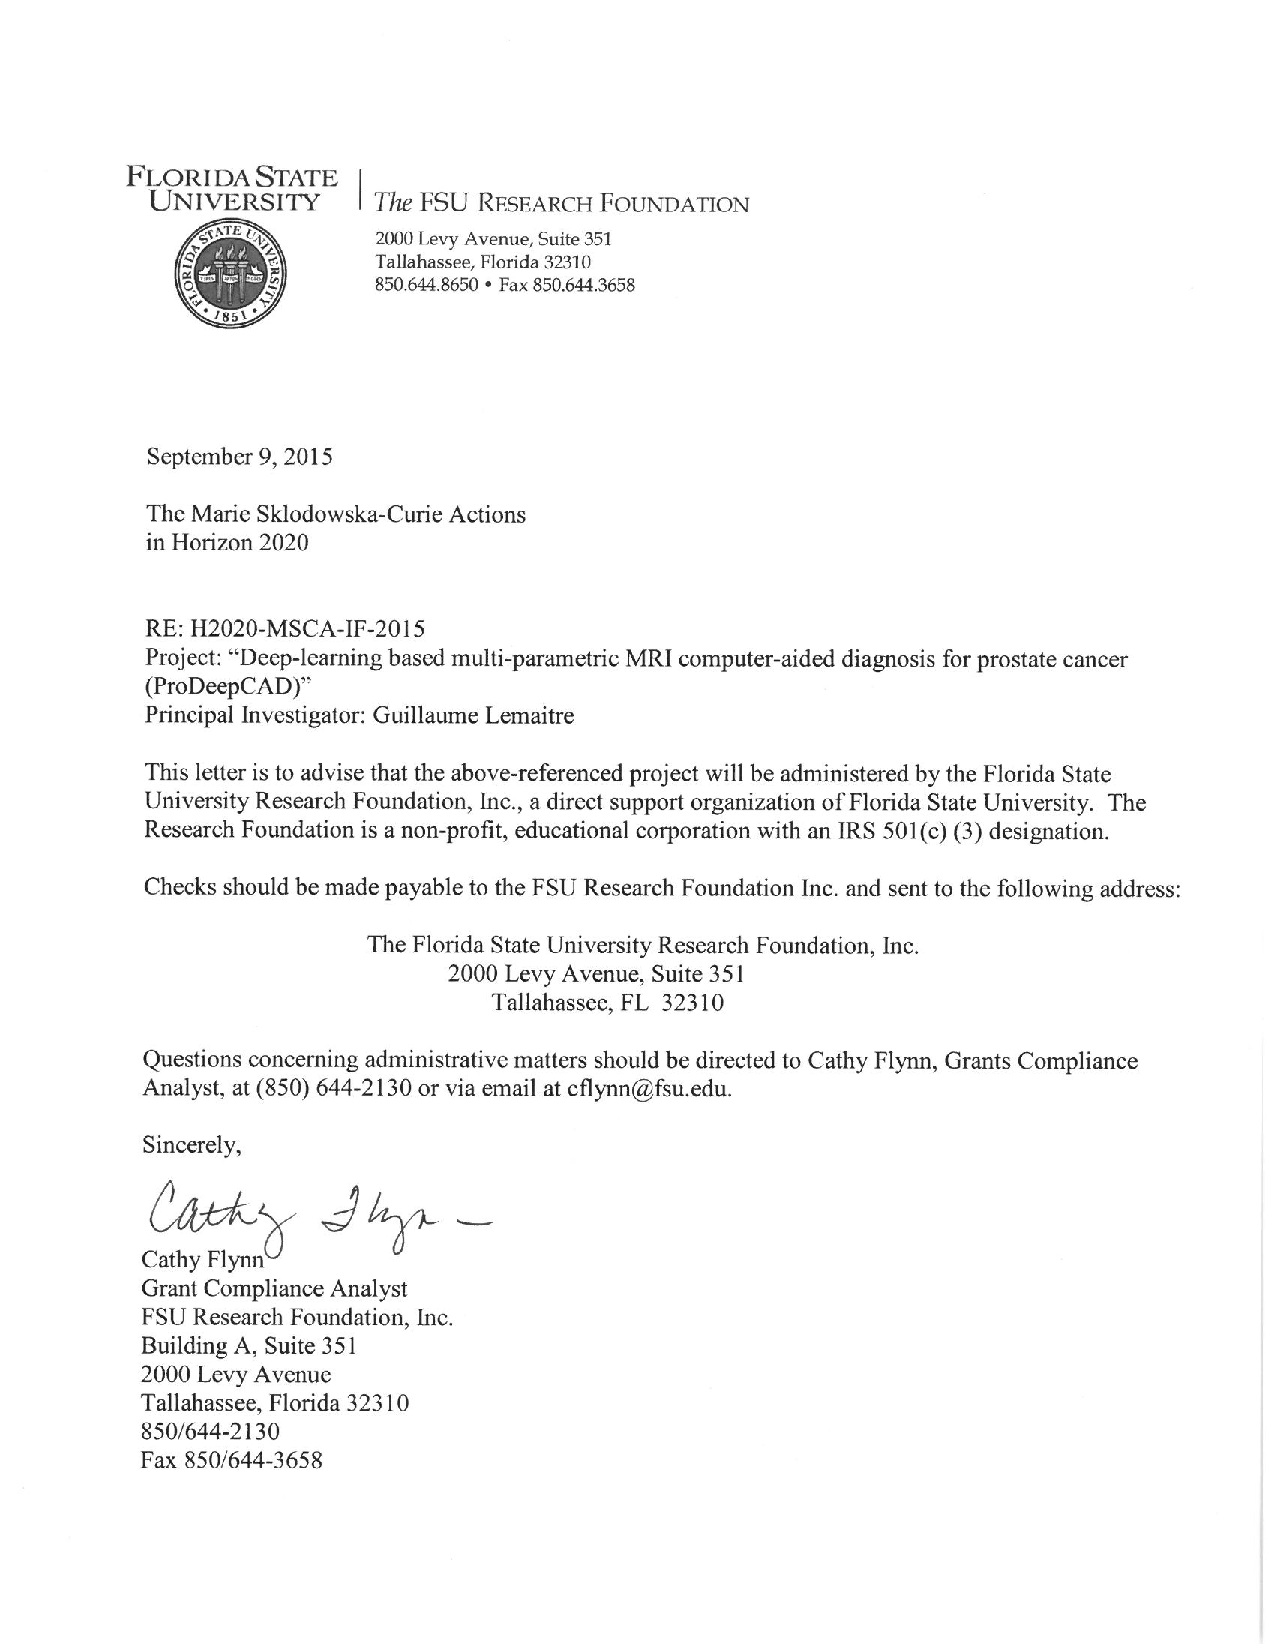
\includegraphics[height=.96\textheight]{./content/ethical/lemaitre.pdf}
\end{figure}
                      % the file wihtout .tex

% \include*{content/other/other}
% \printbibliography

\newpage
\vspace{15mm}
\begin{center}


        \Large{


        \textbf{ENDPAGE}

          \vspace{15mm}
          MARIE SK\L{}ODOWSKA-CURIE ACTIONS\\
          \vspace{1cm}

          \textbf{Individual Fellowships (IF)}\\
          \textbf{Call: H2020-MSCA-IF-2016}
          \vspace{2cm}

          PART B
          \vspace{2.5cm}

          ``\proposalAcronym''\\
          \vspace{1cm}
          ``Deep-learning based multi-parametric MRI computer-aided diagnosis for prostate cancer''
          \vspace{1cm}

          \textbf{This proposal is to be evaluated as:}
          \vspace{.5cm}

          \textbf{[Standard GF]}
        }

  \end{center}
\vspace{1cm}

\end{document}
